\section{Architecture du site web}
\label{sec:Architecture}

\paragraph{}Dans cette section, nous pr�sentons l'architecture du site web r�alis�.
\subsection{Architecture physique}
\label{sec:archiphys}

\paragraph{} L'architecture physique du site web est divis� en 4 parties:
\begin{itemize}
\item Les pages web: � la racine du site web
\item Les fonctions php: dans les librairies dans le dossier "lib" ainsi que dans le dossier "include"
\item Les differentes ressources: dans les dossier "res" et "img"
\item Le style du site: dans les dossier "css" et "police"
\end{itemize}

\begin{figure}[H]
	\centering
		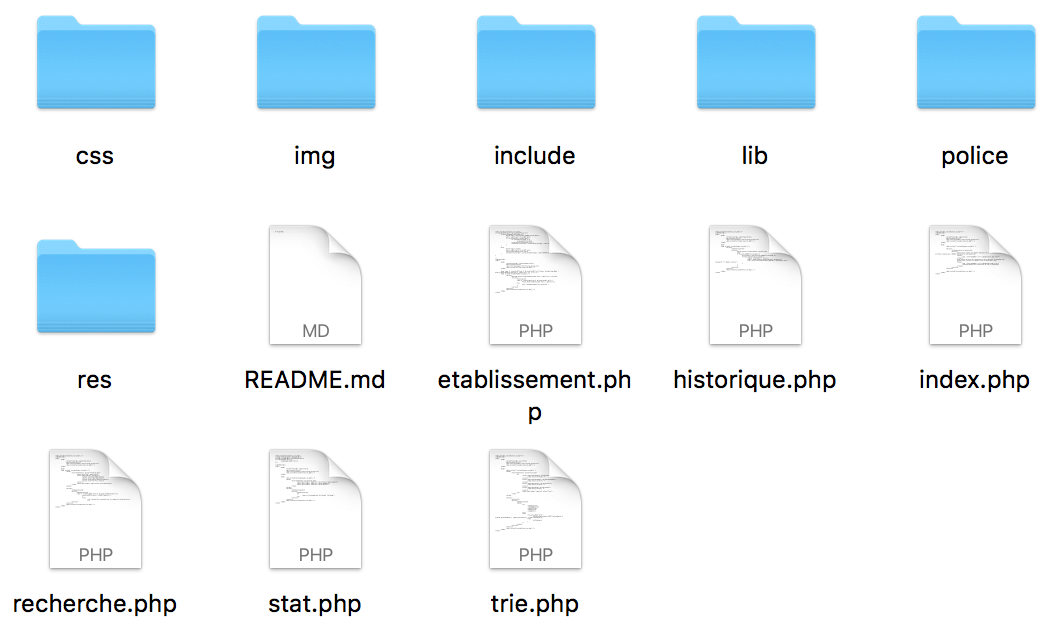
\includegraphics[width=15cm,height=10cm]{img/archi_phys.png}
		\caption{Architecture Physique du site web}
	\label{fig:archiphys}
\end{figure}

\subsection{Architecture Logique}
\label{sec:archilog}

\paragraph{}Le site web est construit de telle mani�re � ce que chaque page soit accessible � partir de n'importe quelle autre page.

\subsection{L'unit� d'adressage}
\label{sec:spec3}

\paragraph{} 

\subsection{L'unit� de contr�le}
\label{sec:spec4}

\paragraph{} Le principe de fonctionnement d'une unit� de contr�le est de lire le contenu du registre d'instruction, de le d�coder et d'en d�duire le positionnement des diff�rents signaux de l'architecture (ALU, sources, destinations, acc�s m�moire).